\documentclass[10pt,twocolumn]{article}
\usepackage[a4paper,margin=1.75cm,columnsep=0.65cm]{geometry}
\usepackage[T1]{fontenc}
\usepackage[utf8]{inputenc}
\usepackage{mathptmx}
\usepackage{amsmath,amssymb,graphicx,booktabs,array,multirow}
\usepackage{microtype}
\usepackage[font=small,labelfont=bf]{caption}
\usepackage[numbers,sort&compress]{natbib}
\usepackage[dvipsnames]{xcolor}
\usepackage[colorlinks=true,linkcolor=MidnightBlue,citecolor=MidnightBlue,urlcolor=MidnightBlue]{hyperref}
\usepackage{enumitem}
\usepackage{fancyhdr}
\hypersetup{pdftitle={Gated Dual-State Memory for Robust Temporal Processing in Spiking Neural Networks},pdfauthor={Anonymous authors},pdfsubject={Research manuscript draft},pdfkeywords={spiking neural networks, shared memory, gated dual-state memory, temporal robustness}}
\raggedbottom
\setlength{\parskip}{2pt}
\setlength{\textfloatsep}{13pt plus 2pt minus 2pt}
\setlength{\floatsep}{10pt}
\setlength{\emergencystretch}{1.5em}
\setcounter{topnumber}{3}\setcounter{totalnumber}{4}
\renewcommand{\topfraction}{.92}\renewcommand{\textfraction}{.07}
\pagestyle{fancy}\fancyhf{}\fancyhead[L]{\small Gated Dual-State Memory}\fancyhead[R]{\small Research draft}\fancyfoot[C]{\thepage}
\renewcommand{\headrulewidth}{.3pt}
\makeatletter\let\tableinput\@@input\makeatother
\newcommand{\R}{\mathbb{R}}
\newcommand{\CE}{\operatorname{CE}}
\newcommand{\relu}{\operatorname{ReLU}}
\newcommand{\diag}{\operatorname{diag}}
\newcommand{\ind}{\mathbb{I}}
\title{\vspace{-1.1cm}\textbf{Gated Dual-State Memory for Robust Temporal Processing\newline in Spiking Neural Networks}}
\author{Anonymous authors}
\date{Manuscript draft --- November 5, 2026}
\begin{document}
\maketitle
\begin{abstract}
Compact shared memory extends the temporal reach of spiking neural networks, but a continuously updated state can lose useful information during pauses and irrelevant input. We introduce gated dual-state memory (GDSM), a shared-memory architecture that separates an always-updated candidate state from a selectively updated stable state. A vector input projection increases the information entering memory, while causal, dimension-wise gates control delayed writing and independent read weights combine the two states with the fast spiking pathway. We evaluate this design on spiking speech, event-camera gestures, and sequential and permuted MNIST, distinguishing whole-sequence classification from classification after an appended interruption. With matched training within each comparison, GDSM achieves 52.79\% endpoint accuracy on Spiking Speech Commands after 120 Poisson-noise frames, versus 3.91\% for the original dual-memory-pathway model. On DVS Gesture, accuracy after 80 silent frames increases from 19.70\% to 70.83\%. Across three training seeds, sequential MNIST reaches 78.68\% after an unseen 160-frame pause, versus 8.69\% for DMP. SHD controls separate input bandwidth, write protection, and explicit noise supervision. A fixed-point memory-core implementation reproduces 117,056 reference values exactly in a 944-step RTL replay. The results establish gated stable-state updating as an effective mechanism for retaining class information through interruptions, with measurable computation costs and a remaining trade-off between retention and rapid context switching.
\end{abstract}
\noindent\textbf{Keywords:} spiking neural networks; shared memory; selective state updates; temporal robustness; neuromorphic computation.

\section{Introduction}
An event-driven classifier should often retain its interpretation after the event itself has ended. A gesture may be followed by inactivity, a spoken command by background activity, and a sequential sensor measurement by a temporary interruption. Correctly averaging predictions over the original event does not establish this ability: the average can remain correct even after the current network state has forgotten the class. Retention therefore needs an explicit evaluation at the end of the interruption.

Dual memory pathways (DMP) address the short temporal horizon of conventional spiking neurons by adding a small, shared state to each layer~\cite{dmp}. A fixed Legendre recurrence summarizes past input and supplies a slow current to the fast spiking pathway. This organization is attractive because the memory dimension can be much smaller than the layer width. Its continuous update, however, couples two different requirements: incorporating new evidence and preserving a useful existing representation. Both silence, through autonomous state evolution, and unrelated activity, through new drive, can change the stored representation.

We study a simple separation of these roles. A \emph{candidate} state continues to process the input, while a \emph{stable} state receives selected, delayed updates. A learned gate uses current input statistics and past evidence to decide which coordinates to write. The fast pathway and the candidate remain available to the classifier when stable memory is held. We also replace the scalar input bottleneck of the original shared state with a vector projection, allowing different coordinates to receive different combinations of input features. We call this architecture \emph{gated dual-state memory} (GDSM).

The objective is robust shared memory, rather than a new general-purpose gating primitive. The central empirical question is whether a compact state shared across a spiking layer can preserve discriminative information through interruptions while remaining usable for ordinary classification. Our study contributes: (i) a concrete candidate--stable memory design with vector drive and separate reads; (ii) controlled classification and endpoint-retention experiments across speech, event vision, and 784-step image sequences, including held-out interruption lengths; and (iii) a fixed-point functional implementation that exposes the cost and conditional reuse enabled by stable memory. SHD ablations explain why write protection alone is insufficient, and context-switching tests identify where retention remains costly.

\section{Related work}
\paragraph{Gated and structured recurrent memory.}
LSTM and GRU established learned retention and update gates in recurrent networks~\cite{lstm,gru}. Legendre memory units encode temporal information using a structured linear dynamical system~\cite{lmu}; HiPPO and S4 develop related polynomial-projection and state-space approaches~\cite{hippo,s4}. Input-dependent selection is also central to Mamba~\cite{mamba}. GDSM uses this established idea of selective state updating. Its particular design retains the DMP layer-shared organization, keeps the structured candidate dynamics active during write closure, and reads candidate and stable states separately into a spiking population.

\paragraph{Temporal memory in spiking networks.}
Surrogate-gradient learning makes recurrent spiking dynamics accessible to gradient-based optimization~\cite{surrogate}, with software support such as SpikingJelly~\cite{spikingjelly}. Gated LIF neurons and two-compartment models modify neuronal dynamics to improve temporal processing~\cite{glif,tclif}. DMP instead shares a compact slow state across a layer~\cite{dmp}. Our intervention is in that shared memory branch. The main comparisons retain the same fast backbone and compare a feedforward SNN (FSNN), scalar-drive DMP, and GDSM. Thus the study tests the benefit and cost of the complete shared-memory design; the SHD experiments provide more targeted component controls.

\section{Gated dual-state memory}
\label{sec:method}
\subsection{From a scalar summary to vector drive}
Let $z_t\in\R^M$ denote a layer input and let the layer contain $N$ spiking neurons. The original DMP branch uses a scalar drive and a $d$-dimensional recurrent state,
\begin{align}
 x_t &= \relu(w_u^\top z_t+b_u),\\
 h_t &= \bar A h_{t-1}+\bar B x_t,
\end{align}
where $\bar A\in\R^{d\times d}$ and $\bar B\in\R^{d\times1}$ are fixed discretized Legendre matrices. A learned read projection maps $h_t$ into the neural current. The state can encode temporal structure despite its scalar input, but every new frame enters through the same one-dimensional projection.

GDSM instead uses
\begin{align}
 u_t &= \relu(W_u z_t+b_u)\in\R^d,\label{eq:drive}\\
 p_t &= \bar A p_{t-1}+D u_t,\label{eq:candidate}
\end{align}
where $W_u\in\R^{d\times M}$ and $D$ is a fixed diagonal scaling matrix. The transition matrix is inherited from DMP; the vector-driven recurrence is an adaptation of that dynamics rather than an assertion that each coordinate remains the original scalar Legendre projection. The vector projection increases the input bandwidth of the memory branch. This is especially relevant when input channels carry different frequency or spatial features.

\begin{figure*}[t]
 \centering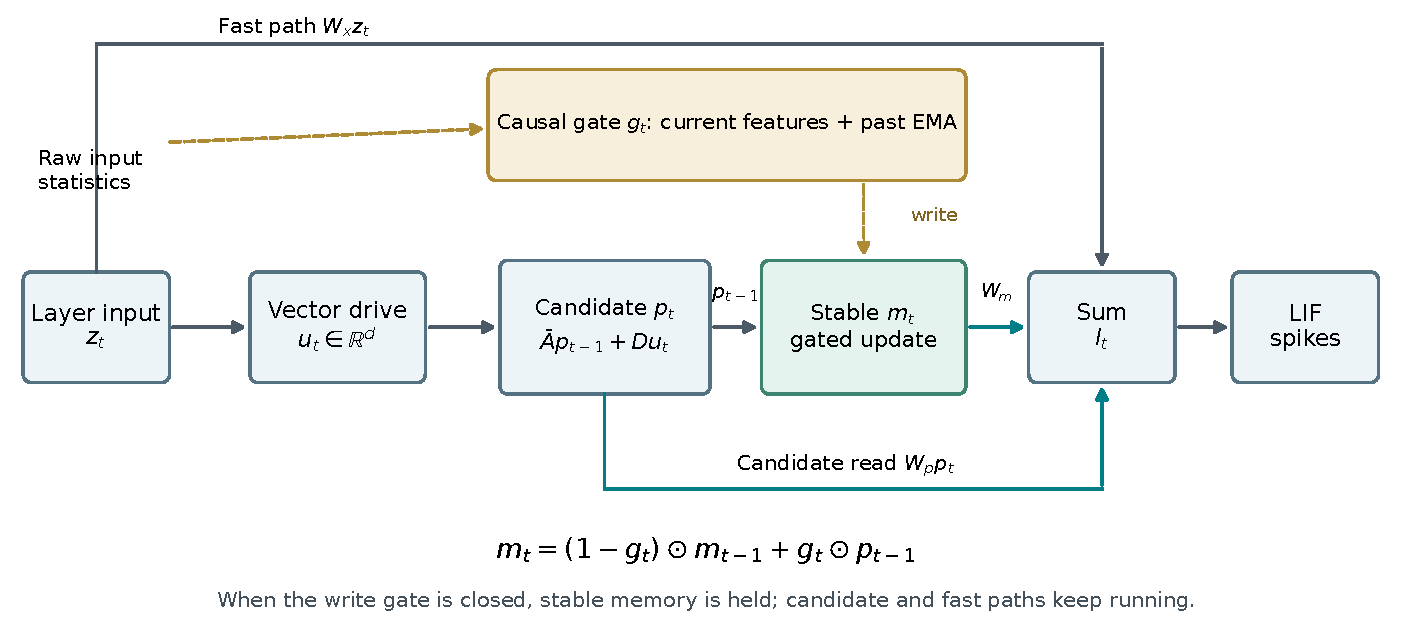
\includegraphics[width=.96\textwidth]{figures/architecture.pdf}
 \caption{GDSM within one spiking layer. The candidate $p_t$ continuously integrates vector-projected input. A causal gate writes the previous candidate to stable memory $m_t$. Independent projections read both states into the fast pathway. Gate closure preserves $m_t$ while candidate and LIF computation continue. The raw-input statistics branch is shared across memory layers, with separate gate outputs.}
 \label{fig:architecture}
\end{figure*}

\subsection{Delayed writing and independent reading}
The stable state evolves as
\begin{equation}
 m_t=(1-g_t)\odot m_{t-1}+g_t\odot p_{t-1},\qquad g_t\in[0,1]^d.
 \label{eq:commit}
\end{equation}
The gate thus evaluates current evidence before writing the previous candidate. A single-step delay does not by itself reject a long disturbance; protection depends on the learned gate. It does keep newly arriving input from being copied directly into stable memory in the same update.

The layer current is
\begin{equation}
 I_t=W_xz_t+W_pp_t+W_mm_t+b.
 \label{eq:read}
\end{equation}
The three paths have independent weights, followed by the same LIF dynamics as the corresponding backbone. In the main cross-dataset experiments their read coefficients are fixed at one. Candidate and stable memory are shared by the layer, not replicated for every neuron. Their recurrent state cost is $2d$, compared with $d$ for DMP, before gate-feature history and any read cache.

\subsection{Causal write decisions}
For local input $z_t$, we compute four statistics: normalized mean activity, absolute change in mean activity, variance, and positive-input occupancy. Let this feature vector be $f_t$ and its exponentially weighted history be $e_t$:
\begin{equation}
 e_t=\rho e_{t-1}+(1-\rho)f_t,\qquad \rho=0.8.
\end{equation}
The local gate uses the current features and the \emph{previous} history,
\begin{align}
 a_t &= \sigma\!\left(G[f_t;e_{t-1}]+b_g\right),\\
 \tilde g_t &= a_t\odot\ind[a_t\geq\epsilon],\quad \epsilon=0.02.
\end{align}
A small permission MLP uses current raw-input features and their previous EMA to produce a binary, dimension-wise permission $q_t$. The final gate is
\begin{equation}
 g_t=\tilde g_t\odot q_t\,\ind[\|r_t\|_1>0],
 \label{eq:gate}
\end{equation}
where $r_t$ is the nonnegative raw frame. Auditory features include pooled frequency bands, visual features include coarse spatial activity by polarity, and scalar-pixel input uses the four statistics alone. Hard thresholding is used in the forward pass and sigmoid derivatives provide surrogate gradients. Appendix~\ref{app:implementation} specifies feature dimensions and initialization.

The zero-input rule is an explicit, observable-input prior: a fully empty frame cannot change stable memory. It also applies to naturally empty frames, including black pixels in sequential MNIST. It does not require the position of an artificial interruption. Neither time indices, interruption masks, segment lengths nor class labels are inputs to the model. Known query times are used to construct supervised losses and evaluation scores.

\subsection{What closure guarantees}
For a fixed realized gate sequence, the direct coefficient of an old stable coordinate over a length-$L$ interval is
\begin{equation}
 R_j(t,L)=\prod_{k=t+1}^{t+L}(1-g_{k,j}).
 \label{eq:retention}
\end{equation}
A small nonzero gate can still produce substantial decay: a constant $g=0.02$ gives $(0.98)^{80}\approx0.199$. In contrast, exact closure gives $m_{t+L}=m_t$. The complete state also contains the accumulated candidate writes, so $R_j$ measures a direct old-state coefficient, not classification accuracy or the total derivative through the recurrent system.

When every coordinate is closed, the stable read $W_mm_t$ is unchanged and can be cached. Partial coordinate closure alone does not eliminate a dense matrix read in our implementation. This creates a concrete conditional computation opportunity while leaving candidate and fast processing active.

\subsection{Training objective}
All main comparisons use ordinary class supervision. Let $o_t$ denote the output score and let $\bar o$ and $\bar o_{20}$ be its whole-sequence and final-20-frame averages. Mixed training uses
\begin{equation}
 \mathcal L_{\mathrm{mixed}}=\tfrac12\CE(\bar o,y)+\tfrac12\CE(\bar o_{20},y).
 \label{eq:loss}
\end{equation}
This teaches both recognition and persistence. SSC uses the same objective in its clean stage; MNIST uses $\CE(\bar o,y)$ for clean training. Gesture starts from clean validation-selected checkpoints and uses Eq.~\eqref{eq:loss} in the controlled fine-tuning stage. SSC, Gesture and MNIST use neither noise-position supervision nor an auxiliary memory classifier.

SHD development experiments additionally use a stable-state auxiliary classification head, enabling us to distinguish useful storage from successful downstream reading. The supervision ablation explicitly compares class-only training, addition of the zero-input rule, and addition of mask-derived gate losses. These variants are reported separately from the main class-supervised transfer studies.

\section{Experimental design}
\label{sec:protocol}
\subsection{Tasks and matched comparisons}
We use four source datasets and five classification tasks: SHD and Spiking Speech Commands (SSC)~\cite{shd}, DVS Gesture~\cite{gesture}, and sequential and permuted sequential MNIST (S-MNIST and PS-MNIST)~\cite{mnist}. SHD provides architecture and mechanism diagnostics. SSC, Gesture and the two MNIST orderings provide the main comparisons of the frozen architecture. Table~\ref{tab:protocol} summarizes their scale.

For each main experiment, FSNN, DMP and GDSM share the backbone width, data, training schedule, input realizations and classification objective. SSC and MNIST also share the initial fast-path and output weights; GDSM's vector drive is initialized from the scalar DMP drive. Gesture uses each model's own historical clean checkpoint, followed by identical mixed fine-tuning inputs and update counts. Equal $d$ is a comparison at the same candidate-state dimension, not at equal total parameters. We report parameter counts and use a nearly parameter-matched SHD control to isolate the vector bottleneck.

\begin{table*}[t]
\centering\small
\caption{Main experimental protocols. The two MNIST tasks use the same images with different orderings. $T$ is the number of input frames; $d$ is the per-layer candidate dimension. ``50 + 20'' for Gesture means a checkpoint selected by validation within 50 clean epochs, followed by 20 fixed mixed epochs.}
\label{tab:protocol}
\begin{tabular}{lrrrrll}
\toprule
Task & Train / validation / test & Classes & $T$ & $d$ & Backbone & Clean + mixed epochs\\
\midrule
SSC & 75,466 / 9,981 / 20,382 & 35 & 250 & 30 & $140\to128\to128\to35$ & $40+12$\\
DVS Gesture & 901 / 176 / 264 & 11 & 100 & 40 & Conv32--Conv64--FC256--11 & $50+20$\\
S-MNIST & 54,000 / 6,000 / 10,000 & 10 & 784 & 40 & $1\to200\to200\to10$ & $50+12$\\
PS-MNIST & 54,000 / 6,000 / 10,000 & 10 & 784 & 40 & $1\to200\to200\to10$ & $50+12$\\
\bottomrule
\end{tabular}
\end{table*}

\subsection{Interruption and retention protocols}
We distinguish two tests. In \emph{middle interruption}, a silent or Poisson-noise segment is inserted halfway through the input, after which the original sequence resumes. Accuracy is computed from the average score over the entire extended sequence. In \emph{tail retention}, the same type of segment is appended after the full input, and classification uses only the last 20 frames at the end of that segment. The original class remains the target. We also report the last-20-frame accuracy at the clean endpoint ($L=0$), which separates initial endpoint quality from subsequent forgetting.

SSC and MNIST mixed training sample clean, silent and noisy inputs with equal probability, using interruption lengths 40 and 80 and either middle or tail placement. Evaluation adds an unseen length: 120 for SSC and 160 for MNIST. SSC noise has a fixed Poisson rate of 0.25 per channel per frame. MNIST noise is Poisson with rate 0.1, clipped to $[0,1]$. Gesture uses lengths 20, 40 and 80, with a training-calibrated event-density noise rate (1$\times$); 3$\times$ noise is an intensity-shift test. Identical noise realizations are used across the three model families.

Auditory and gesture inputs are normalized within known event segments. Thus the inference recurrence is causal over the encoded frames, while preprocessing uses the segment boundaries. These experiments measure retention in constructed streams, rather than end-to-end recognition of unsegmented raw recordings. The longest main evaluation sequence is 944 pixel steps.

\subsection{Repetitions and reporting}
S-MNIST and PS-MNIST each use three independent training seeds (42, 43 and 44), with all 18 models frozen before official test evaluation. Values with $\pm$ denote sample standard deviation across training seeds. SSC uses one training seed (801). Gesture uses one fine-tuning seed (701); its three noise seeds are averaged and are not treated as independent trained models. The SHD supervision study uses three fine-tuning seeds per configuration.

For SSC and Gesture, paired confidence intervals use speaker- or subject-cluster bootstrap, respectively. These intervals quantify test-population sampling conditional on the trained models. MNIST paired intervals use the three per-seed differences and a Student-$t$ interval with two degrees of freedom. We report the entire fixed seed set and final scheduled checkpoints. Appendix~\ref{app:reproduce} details the evidence organization and additional settings.

\section{Results}
\subsection{Classifying the event and retaining its label}
Table~\ref{tab:clean} reports whole-sequence clean classification. GDSM improves SSC accuracy over DMP under both stages and reaches 58.83\% after mixed training. On Gesture, both memory models reach 86.74\%. The clean-trained MNIST comparisons show high accuracy for both memory models, with mean GDSM improvements of 0.71 percentage points on S-MNIST and 1.35 on PS-MNIST. Their paired 95\% intervals include zero; the primary benefit in this study is retention rather than a decisive gain on clean MNIST.

The distinction between whole-sequence and endpoint scoring is consequential. After mixed training, SSC DMP achieves 47.89\% clean whole-sequence accuracy but only 11.05\% at the clean endpoint. GDSM reaches 58.83\% and 56.52\%, respectively. Its advantage therefore has two components: a better endpoint representation and better preservation of that representation. Comparing tail accuracy only with whole-sequence accuracy would conflate them.

\begin{table*}[t]
\centering\small
\caption{Clean whole-sequence accuracy (\%). ``Clean'' is the clean-training checkpoint; ``Mixed'' is the subsequent interruption-trained checkpoint. MNIST values are mean $\pm$ sample SD over three training seeds; SSC and Gesture are single trained-model results.}
\label{tab:clean}
\begin{tabular}{llrrr}
\toprule Task & Training stage & FSNN & DMP & GDSM\\\midrule
\tableinput{tables/clean.tex}
\bottomrule
\end{tabular}
\end{table*}

\subsection{Stable retention through long interruptions}
Table~\ref{tab:retention} and Fig.~\ref{fig:retention} show tail retention after matched mixed training. On SSC, GDSM retains 54.93\% accuracy after 120 silent frames and 52.79\% after 120 noise frames. These are drops of only 1.59 and 3.73 points from its clean endpoint. DMP reaches 3.52\% and 3.91\%, respectively. The paired GDSM--DMP gains are 51.41 points for silence (95\% speaker-cluster interval $[49.49,53.25]$) and 48.88 points for noise ($[46.96,50.73]$). The nearly flat GDSM curves from 40 to 120 frames demonstrate retention beyond the interruption lengths used for training.

Gesture provides a complementary comparison because the two memory models have similar clean endpoint accuracy: 85.61\% for DMP and 86.36\% for GDSM. After an 80-frame pause, DMP falls to 19.70\% while GDSM retains 70.83\%. At the trained noise intensity, the corresponding values are 26.52\% and 47.47\%. The paired gains are 51.14 points for silence ($[42.93,57.27]$) and 20.96 points for noise ($[11.07,28.40]$), using subject-cluster intervals. Here, the retention difference cannot be explained by a large initial endpoint gap.

On the full 784-step pixel sequences, GDSM also preserves more information through the unseen 160-frame tail. S-MNIST silence accuracy is $78.68\pm15.74$\%, compared with $8.69\pm5.36$\% for DMP. PS-MNIST reaches $56.43\pm17.28$\%, compared with $14.12\pm0.46$\%. Noise is harder: GDSM reaches $32.03\pm15.51$\% and $28.02\pm12.89$\%, respectively. All three seeds improve over DMP on each of these four tail conditions, but the magnitudes vary substantially; only the S-MNIST silence gain excludes zero under the three-seed $t$ interval. The cross-task pattern is strong preservation through inactivity, with more variable preservation through active distractors.

\begin{table*}[t]
\centering\small
\caption{Endpoint classification after the longest appended interruption (\%), using the same last-20-frame readout at $L=0$ and after the gap. All models have completed mixed training. Length 120 for SSC and 160 for MNIST were absent from training; Gesture noise is 1$\times$.}
\label{tab:retention}
\begin{tabular}{llrrrr}
\toprule Task & Model & $L$ & Clean endpoint & Silence endpoint & Noise endpoint\\\midrule
\tableinput{tables/retention.tex}
\bottomrule
\end{tabular}
\end{table*}

\begin{figure*}[t]
\centering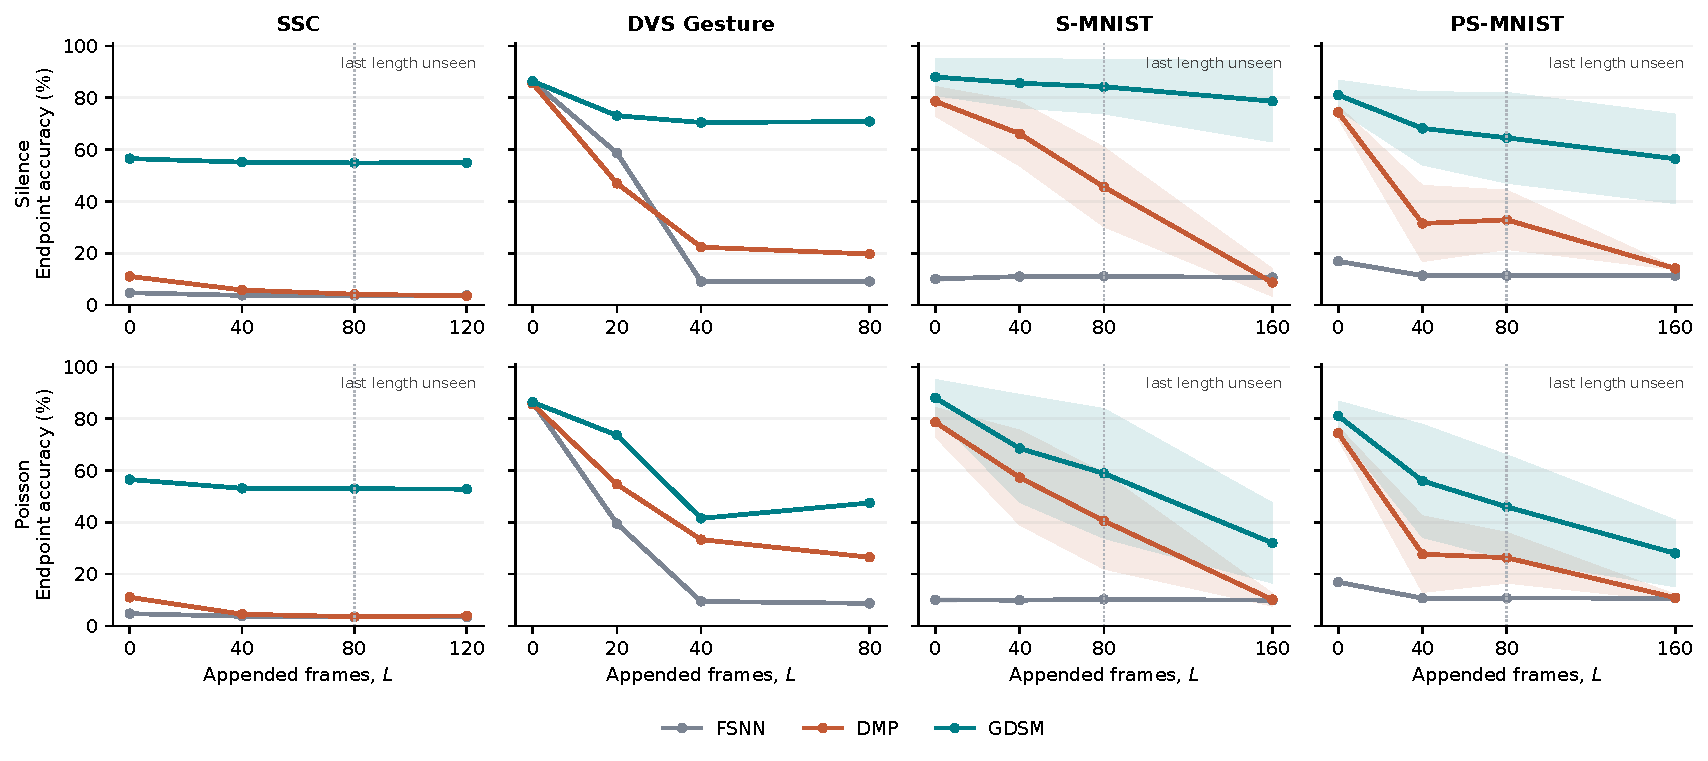
\includegraphics[width=\textwidth]{figures/retention.pdf}
\caption{Tail-retention curves after mixed training. The point at $L=0$ uses the clean endpoint, not the whole-sequence mean. Shading is one training-seed SD for the two MNIST tasks; SSC and Gesture have one trained model per family. Gesture noise values average three paired noise realizations. The dashed lines mark the largest trained length where a longer unseen length is tested.}
\label{fig:retention}
\end{figure*}

\subsection{Recovery during a sequence and the role of training}
Middle interruptions are a different problem: later task input can replenish the state. GDSM exceeds DMP on all six SSC middle conditions; for the unseen length 120, its accuracy is 51.79\% versus 36.66\% under silence and 50.94\% versus 42.05\% under noise. On Gesture, it exceeds DMP in seven of nine middle conditions, including 54.17\% versus 19.19\% for 3$\times$ noise at length 80. FSNN reaches 64.27\% in that strong-noise condition, showing that memory can also retain harmful context. Moreover, the final-20-frame recovery score of GDSM is 18.31 points below DMP there, despite its higher whole-sequence average. The two readouts answer different questions.

On MNIST, middle-interruption gains are smaller and mixed. At length 160, GDSM's whole-sequence accuracy is 2.17 points below DMP for S-MNIST silence and 2.42 points below for PS-MNIST silence; its noise differences are $+3.93$ and $+0.68$ points. Appendix~\ref{app:middle} reports every middle condition. The architecture is most beneficial when the task demands retaining a completed observation through a gap, rather than simply averaging predictions across an interrupted sequence.

Training on disturbances is necessary for the noise results. Clean-only GDSM reaches just 11.47\% on SSC tail noise of length 120, rising to 52.79\% after mixed training. The corresponding clean-only values at length 160 are $11.99\pm1.09$\% for S-MNIST and $11.82\pm0.94$\% for PS-MNIST. By contrast, the zero-input rule already supports substantial silence retention before mixed training. The architecture provides a protected storage mechanism; class-supervised disturbance exposure teaches how to use it.

The endpoint objective also has a cost for the short-memory FSNN. Its S-MNIST clean whole-sequence accuracy falls from $45.71\pm2.10$\% to $14.84\pm1.37$\% after mixed training. The identical objective is a controlled comparison, but it is not equally compatible with every architecture. We therefore preserve the clean-stage comparison and interpret the mixed stage as a joint recognition-and-retention task.

\subsection{Why vector drive and selective writes both matter}
\label{sec:ablation}
SHD offers targeted evidence on the mechanism. In the protected-memory recipe, scalar, wide-scalar and vector variants share independent candidate/stable reads and an auxiliary memory loss. The wide-scalar model first expands input to $d$ coordinates and then compresses it back to one drive. Its parameter count closely matches the vector model. Table~\ref{tab:capacity} shows that removing the final scalar bottleneck improves both the auxiliary endpoint representation and the main SNN's retention. At $d=30$, vector drive reaches 66.70\% mean L80 retention versus 59.76\% for the slightly larger wide-scalar control. At $d=10$, the corresponding values are 51.88\% and 47.46\%.

A separate three-seed scalar--vector comparison gives mean retention gains of 14.36 points at $d=10$ and 12.46 at $d=30$. Without protection, the vector model retains only 23.98\% and 38.25\% in the single-seed controls, versus 51.88\% and 66.70\% when protected. These results support complementary roles: input bandwidth determines what can be stored, and selective writing determines what survives. This historical capacity experiment used explicit gate supervision, which is separated from the next ablation.

\begin{table}[t]
\centering\small
\caption{SHD capacity control, seed 501. ``Aux.'' reads stable memory at the clean word endpoint; ``Ret.'' is main-SNN accuracy averaged over silence and noise L80 tails. All rows use the same historical protected recipe, including noise-derived gate losses.}
\label{tab:capacity}
\begin{tabular}{rlrrr}
\toprule $d$ & Input drive & Parameters & Aux. (\%) & Ret. (\%)\\\midrule
10 & Scalar & 45,050 & 48.19 & 40.15\\
10 & Wide scalar & 47,502 & 56.67 & 47.46\\
10 & Vector & 47,480 & 68.24 & 51.88\\\addlinespace
30 & Scalar & 57,410 & 68.82 & 52.65\\
30 & Wide scalar & 65,302 & 69.57 & 59.76\\
30 & Vector & 65,240 & 81.05 & 66.70\\
\bottomrule
\end{tabular}
\end{table}

\subsection{Supervision and the retention--switching trade-off}
Table~\ref{tab:supervision} compares three SHD training arms with matched initialization, inputs and optimization. At $d=30$, adding the zero-input rule increases silence retention from 29.52\% to 67.82\%. Adding noise-position-derived gate losses on top of the rule changes noise retention only from 60.16\% to 60.81\%. Thus the strong $d=30$ result does not require an explicitly supervised noise detector. At $d=10$, the same supervision adds 7.18 points under noise, indicating that its value depends on capacity.

The gate-only retention coefficient and class retention are different. For $d=30$ with task supervision and the zero rule, the mean L80 noise coefficient in Eq.~\eqref{eq:retention} is 0.706, while the auxiliary head retains 74.26\% class accuracy. Requiring every coordinate to retain 80\% of its old coefficient is therefore neither achieved nor necessary for these aggregate classification results.

Preserving context also makes switching consequential. In SHD streams with two different word labels, the fixed-read $d=30$ model recognizes the new word at 12.22\% during its first 20 frames and at 71.72\% during its last 20 frames. It still predicts the old label in 27.72\% of the early windows. A final frozen-memory readout experiment trained the new-word 20/40-frame queries without altering candidate states, stable states or write gates. Dynamic prefix reading reached 12.69\% at 20 frames, while standard-noise retention changed from 60.16\% to 61.50\%. The improvement was small. A boundary-reset diagnostic improves early recognition, but early word fragments also contain limited class information. The remaining problem is to use new evidence rapidly without discarding protected context; more aggressive forgetting is not established as the solution.

\begin{table*}[t]
\centering\small
\caption{SHD supervision ablation (mean $\pm$ SD, three fine-tuning seeds). All arms use vector drive and identical class/auxiliary classification losses. ``Gate labels'' adds mask-derived opening and cumulative-leakage losses. Columns are main-SNN accuracies (\%).}
\label{tab:supervision}
\begin{tabular}{rlllll}
\toprule $d$ & Training arm & Clean mean & Silence L80 & Noise L80 & New word mean\\\midrule
10 & Task losses & $85.62\pm2.06$ & $31.38\pm3.19$ & $41.64\pm9.83$ & $73.28\pm2.51$\\
10 & Task + zero rule & $86.31\pm1.11$ & $58.42\pm4.47$ & $46.29\pm8.23$ & $72.97\pm1.60$\\
10 & Task + zero rule + gate labels & $86.10\pm1.85$ & $60.38\pm4.03$ & $53.47\pm4.17$ & $69.05\pm1.82$\\\addlinespace
30 & Task losses & $87.38\pm0.98$ & $29.52\pm6.19$ & $56.96\pm12.77$ & $75.89\pm1.27$\\
30 & Task + zero rule & $87.99\pm0.87$ & $67.82\pm5.48$ & $60.16\pm8.76$ & $75.63\pm1.59$\\
30 & Task + zero rule + gate labels & $87.99\pm0.19$ & $66.84\pm7.17$ & $60.81\pm13.50$ & $73.29\pm0.27$\\
\bottomrule
\end{tabular}
\end{table*}

\section{Hardware realization and cost}
\label{sec:hardware}
\subsection{Functional fixed-point implementation}
We extend the public DMP Chisel project with a separate GDSM memory core. The core implements vector ReLU drive, the full candidate transition, delayed stable updates, local gates, a scalar-pixel permission MLP, independent reads and a stable-read cache. It produces the memory current to be supplied to the fast/LIF pathway. The implementation uses signed 24-bit Q11.12 values, widened intermediate products, arithmetic right shifts and saturation. A 257-entry sigmoid table covers $[-8,8]$ in steps of $1/16$.

All 25 original project tests pass. Seven additional tests compare the new core with an independent integer reference, covering silence, noise, input changes, delayed writing, partial closure, saturation, random inputs and reset. A separate trained-weight test checks the exported Python reference against the Scala reference. Finally, native Verilator replays the delivered RTL for a real S-MNIST checkpoint: 784 pixels followed by 80 silent and 80 noisy steps. All 117,056 checked fixed-point values match over the 944-step trace. This verifies the memory branch; it is not an end-to-end quantized classification result.

The real-weight trace uses the first memory layer at $d=40$ and four read coordinates. Relative to the floating-point reference, mean absolute errors are 0.00548 for $p$, 0.00508 for $m$, and 0.03341 for the memory current. Gate-open decisions agree in 37,759 of 37,760 coordinate--time pairs. Functional fixed-point correctness and floating-point numerical agreement are thus separately measured.

\subsection{Model-level resource accounting}
Figure~\ref{fig:hardware} places the implementation cost in the context of the full Gesture network. On clean inputs, effective network multiply--accumulate counts increase from 63.212 million for DMP to 67.196 million for GDSM per sample, an overhead of 6.30\%. With an appended L80 silent interval, DMP requires 64.159 million effective MACs and cached GDSM 68.455 million, an overhead of 6.70\%. Stable-read caching reduces GDSM's dense count from 69.274 million to 68.455 million in this condition, saving 1.183\% of full-network work and 4.390\% of memory-layer work.

\begin{figure}[t]
\centering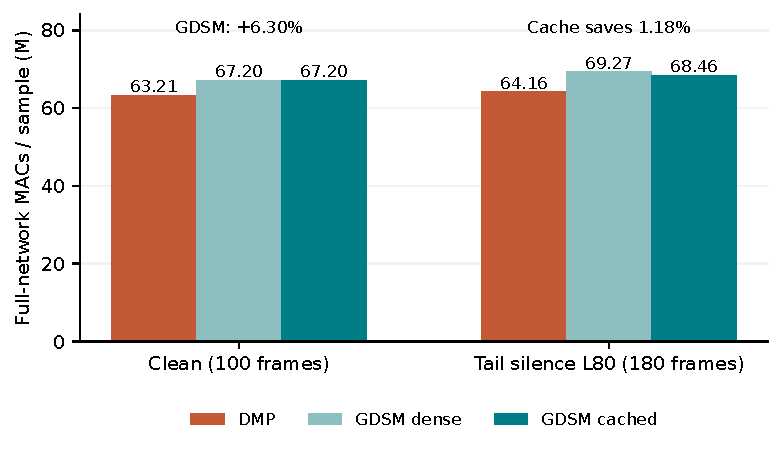
\includegraphics[width=\columnwidth]{figures/full-network-macs.pdf}
\caption{\textbf{Full-network effective MACs on DVS Gesture}, averaged over 264 test samples. The zero-based axis includes convolutional and memory-layer MACs; output-layer synaptic operations are counted separately in the source accounting. Clean-input overhead is 6.30\%; caching saves 1.183\% of dense GDSM MACs during the L80 tail-silence test. These are activity-based operation estimates, not measured full-network cycles or energy.}
\label{fig:hardware}
\end{figure}

GDSM has 66,495 trainable parameters on SSC versus 47,281 for DMP, and 86,778 on MNIST versus 59,213. The corresponding Gesture counts are 1,259,395 and 1,085,356. These model-level costs accompany the retention improvements reported in Table~\ref{tab:retention}.

\subsection{What stable-state reuse saves}
At the memory-core level, full gate closure allows the stable read to be reused while candidate and gate computation continue. With 32 read outputs, caching reduces GDSM processing cycles on closed steps by 23.53\% at $d=10$ and 14.81\% at $d=30$. Appendix~\ref{app:cycles} reports the local cycle counts and matched scalar-DMP schedule separately from the full-network MAC comparison.

On the trained 944-step trace with four read coordinates, 818 stable reads are skipped. Memory-core processing cycles fall from the dense counterfactual of 188,800 to 185,528, a 1.73\% reduction. This measures the benefit of reuse in the implemented schedule while accounting for the stages that continue to execute.

The implementation establishes functional correctness and conditional computation reuse. Physical energy characterization requires the process libraries, SRAM macros and post-layout flow used in the original DMP study~\cite{dmp} and is left to future implementation work.

\section{Discussion}
The results identify a practical distinction between remembering a sequence well enough to average its outputs and retaining its class after the sequence has stopped. GDSM improves the latter across multiple input modalities. Gesture is particularly informative because clean endpoint performance is closely matched, whereas SSC shows that improving the content available at the endpoint can be as important as reducing later drift. The SHD vector-drive and supervision controls support this two-part interpretation.

The design is most applicable when a classification must remain available through a pause or a familiar background disturbance. It is still a classifier with a persistent internal state, not a transcription system or an associative retrieval database. Its memory stores a compressed, task-trained representation rather than addressable examples. A downstream event-driven application could use the stable state to preserve the last recognized context while the fast and candidate paths respond to new activity.

\paragraph{Future directions.}
Future work should extend retention to unfamiliar noise statistics and improve rapid context switching, building on the stress tests and readout diagnostics in Appendix~\ref{app:uncertainty}. Additional training seeds for SSC and Gesture, together with matched-capacity component studies, would broaden the evidence for transfer and isolate the contributions of the complete architecture.

\section{Conclusion}
We introduced GDSM, a vector-driven candidate--stable memory branch for spiking neural networks. Separating ongoing integration from selective stable updates yields large gains in post-interruption classification on spiking speech, event-camera gestures and long pixel sequences. Component controls show that informative write content and write protection are complementary, while task-supervised comparisons demonstrate that explicit noise-position labels are not required for the main transfer results. Functional RTL reproduces the fixed-point reference and makes the additional cost and cache opportunity explicit. The resulting architecture offers a concrete form of persistent shared memory, with its strongest benefits under inactivity and familiar interference and a clear remaining challenge in rapid context switching.

\paragraph{Data and code availability.}
The datasets are publicly released by their original authors~\cite{shd,gesture,mnist}. The DMP implementation used as the starting point is available at \url{https://github.com/sunpengfei1122/Dual_memory_pathways}. The accompanying manuscript artifact includes the source, plotting scripts, result tables, protocol snapshots and an evidence manifest. Training checkpoints, prediction arrays and the hardware source/replay artifacts are retained in the corresponding experiment archives listed in Appendix~\ref{app:reproduce}.

\bibliographystyle{unsrtnat}
\bibliography{references}

\clearpage
\appendix
\section{Implementation and optimization details}
\label{app:implementation}
\subsection{Structured dynamics and initialization}
The fixed transition is inherited from the public DMP implementation, using zero-order-hold discretization with a unit step. For a memory order $d$ and window parameter $\theta$, the continuous-time matrices are
\begin{align}
 A_{ij}&=\frac{2i+1}{\theta}
 \begin{cases}
 -1,&i<j,\\
 (-1)^{i-j+1},&i\geq j,
 \end{cases}\\
 B_i&=\frac{(2i+1)(-1)^i}{\theta},\quad i,j\in\{0,\ldots,d-1\}.
\end{align}
Zero-order hold produces $\bar A$ and $\bar B$. To initialize vector drive from the scalar branch, let $c_i$ be evenly spaced from 0.5 to 1.5. We initialize row $i$ of $W_u$ and its bias as $c_i$ times the scalar weights and bias, and set $D_{ii}=\bar B_i/c_i$. Since $c_i>0$, the initial vector input contribution equals $\bar Bx_t$. The rows subsequently train independently. The stable read is initialized to zero in the paired SSC and MNIST starts, so it does not introduce an initial output mismatch.

Local gate weights start at zero and bias at $\log(0.95/0.05)$. The permission output weights start at zero and output bias at $+2$ for the task-supervised comparisons, initially allowing writes. Historical protected SHD variants use their separately documented calibrated initialization. These settings distinguish the final implementation from proposals to start with strongly closed gates.

For each local feature calculation, the activity normalization scale is clamped below at 0.05. The four statistics are mean divided by scale, absolute mean change divided by scale, variance divided by squared scale, and occupancy. The previous EMA, not an EMA including future frames, is concatenated with current features. The raw-input permission features are:
\begin{itemize}[leftmargin=*,itemsep=1pt,topsep=3pt]
\item \textbf{Auditory:} four statistics plus 14 mean-pooled groups of 10 channels. Current and previous-EMA features form a 36-dimensional input to a $36\to32\to2d$ ReLU MLP, with a gate slice for each hidden layer.
\item \textbf{Gesture:} four statistics plus $2\times4\times4$ polarity/spatial bins, yielding a $72\to32\to d$ permission MLP. Pooled frame counts are further divided by 16 before computing these permission features.
\item \textbf{MNIST:} four scalar-pixel statistics, yielding an $8\to32\to2d$ MLP after adding history. Variance is zero for the scalar input, but the same feature construction is retained.
\end{itemize}
The hard permission is $q_t=\ind[\ell_t\geq0]$. During backpropagation its derivative is replaced with that of $\sigma(\ell_t)$. The local threshold uses its sigmoid derivative in the same manner. Reset sets neural, memory and feature-history states to zero at the beginning of a sequence; inserted gaps do not reset state.

\subsection{SSC}
SSC uses the complete official training, validation and test splits with disjoint speaker sets. Events are rebinned to 250 frames between each utterance's first and last event. The 700 channels are reduced to 140 by taking the maximum across each consecutive group of five channels. This representation is constructed directly from events, rather than interpolating a shorter frame sequence. Models have two 128-unit LIF hidden layers, threshold 1, time constant 2, dropout 0.2, $d=30$ and $\theta=40$.

Training uses batch size 512, AdamW, weight decay 0.05 and gradient-norm clipping at 1. The 40-epoch clean stage starts at learning rate 0.003; the 12-epoch mixed stage starts at 0.001. Each uses cosine decay to $5\times10^{-5}$. Training also uses channel shifts of up to 12 in either direction. Noise seed 901 generates paired evaluation inputs, with shorter lengths taken as prefixes of the maximum-length noise. The frozen model is evaluated on every one of the 20,382 test utterances in each condition.

\subsection{DVS Gesture}
Gesture uses subjects 1--19 for training and the historical 176-segment validation partition for clean checkpoint selection. Official test subjects 24--29 contribute 264 segments. The data mirror has millisecond timestamp precision. Events are grouped into 100 normalized frames; original-resolution counts are averaged over $4\times4$ spatial blocks, producing two-polarity $32\times32$ inputs. The backbone uses 32- and 64-channel $3\times3$ convolutions, LIF activations and $2\times2$ average pooling, followed by a 256-unit fully connected spiking layer and 11 outputs. The shared memory branch is attached to the 256-unit layer, with $d=40$ and $\theta=300$. Scores are output membrane potentials.

The three models begin mixed training from their own best validation checkpoints within the historical 50 clean epochs. Mixed fine-tuning uses Adam, learning rate $10^{-4}$, batch size 4 and 20 fixed epochs. Input-byte hashes confirm identical augmented batches across models. Noise intensity is derived from training activity only; evaluation includes 1$\times$ and 3$\times$ this rate. This is a 100-frame reconstruction of the described backbone, rather than the original paper's 1,000-frame Gesture protocol.

\subsection{Sequential MNIST}
The official training set is stratified into 54,000 training and 6,000 validation images with split seed 1701. Each image supplies all 784 normalized pixels, one scalar per time step. PS-MNIST uses one fixed permutation generated with seed 1702, shared across splits and training seeds. No patching or temporal downsampling is used. Both tasks use two 200-unit LIF layers, threshold 1, time constant 2, no dropout, $d=40$ and $\theta=300$.

Clean training uses Adam for 50 epochs at learning rate 0.001 on S-MNIST and 0.005 on PS-MNIST. Mixed training uses 12 epochs at 0.0003 for both tasks. Batch size is 512, weight decay is zero and gradient clipping is 1. The paired initialization uses the default linear-layer initialization, rather than the original DMP paper's truncated-normal weights and zero biases. Thus these are controlled implementation comparisons, not identical reproductions of its reported benchmark settings. Evaluation noise uses seed 2701. All 18 training runs finish before any official-test evaluation for this block. The total training time was 7,932.53 seconds on an A100 80 GB, with a further 319.1 seconds for evaluation.

\subsection{SHD development studies}
The architecture studies use 6,245 training utterances, 640 validation utterances and a further 1,271-example confirmation subset drawn from the official training release, with training excluding speakers 0 and 2. Official test evaluation uses all 2,264 utterances. Inputs have 140 channels and 100 normalized frames; the backbone has two 128-unit LIF hidden layers, dropout 0.2 and $\theta=40$. A separate full-training-set DMP baseline reached $91.95\pm0.64$\% clean accuracy over three seeds. It is not the GDSM score and is not directly comparable with the smaller-split streaming experiments.

Content training uses 80 epochs with an auxiliary stable-memory cross-entropy loss of weight 1.0. The supervision ablation then uses 30 epochs, batch size 128, AdamW learning rate 0.001, weight decay 0.05, cosine decay to $5\times10^{-5}$ and gradient clipping at 1. All three arms start from matched class-trained sources with freshly initialized permission networks. Training samples are 25\% single words, 37.5\% middle interruptions and 37.5\% paired words, with silent or rate-0.25 Poisson gaps of 20, 40 or 80 frames and channel shifts up to 12. Paired words come from the same speaker and have different 20-class labels. Labels encode both digit and language, so different labels need not denote different numerical digits.

The historical protected capacity study additionally used noise-detector calibration and explicit opening/leakage objectives. Its wide-scalar control is a two-projection branch $M\to d\to1$, with ReLU after each projection. This study supports the input-bandwidth comparison but is not used as evidence that its gate learned without noise labels. The final task-supervised arm removes those gate losses while retaining class labels and known classification query times.

\section{Full middle-interruption results}
\label{app:middle}
Table~\ref{tab:middle} provides every standard-intensity middle condition after mixed training. Each row uses whole-sequence average scores, including the inserted frames. Gesture's additional 3$\times$ intensity results are in Table~\ref{tab:strong}. They illustrate why average classification and post-interruption recovery should be assessed separately.

\begin{table*}[t]
\centering\small
\caption{Complete middle-interruption accuracy after mixed training (\%). MNIST reports three-seed mean $\pm$ SD; SSC and Gesture report one trained-model result. Gesture Poisson is 1$\times$. The longest length is unseen during training for SSC and both MNIST tasks.}
\label{tab:middle}
\begin{tabular}{llrrrr}
\toprule Task & Interruption & $L$ & FSNN & DMP & GDSM\\\midrule
\tableinput{tables/middle.tex}
\bottomrule
\end{tabular}
\end{table*}

\begin{table}[t]
\centering\small
\caption{Gesture under unseen 3$\times$ noise. Middle tests use whole-sequence mean scores; tail tests use the last 20 frames. Noise realizations are paired and averaged.}
\label{tab:strong}
\begin{tabular}{lrrrr}
\toprule Test & $L$ & FSNN & DMP & GDSM\\\midrule
Middle & 20 & 84.47 & 81.82 & 83.59\\
Middle & 40 & 82.20 & 63.13 & 74.87\\
Middle & 80 & 64.27 & 19.19 & 54.17\\\addlinespace
Tail & 20 & 9.09 & 9.09 & 18.69\\
Tail & 40 & 9.09 & 9.09 & 12.50\\
Tail & 80 & 9.09 & 9.09 & 9.09\\
\bottomrule
\end{tabular}
\end{table}

\section{Additional uncertainty and switching analyses}
\label{app:uncertainty}
\paragraph{Noise-distribution shifts.}
On SHD, the $d=30$ task-supervised model with the zero-input rule retains 6.91\% accuracy under L80 noise concentrated in 28 adjacent frequency channels at rate 1.25, compared with 60.16\% for uniform rate-0.25 noise with the same mean intensity. On Gesture, all three models reach 9.09\% tail accuracy under 3$\times$ noise at L80 (Table~\ref{tab:strong}); these probes distinguish reliable silence protection from generalization to active interference.

\paragraph{MNIST paired effects.}
All four longest-tail comparisons improve in each of the three seeds. The S-MNIST silence differences are 75.34, 50.71 and 83.91 percentage points; noise differences are 17.02, 7.10 and 41.49. PS-MNIST silence differences are 51.31, 22.36 and 53.26 points; noise differences are 24.56, 2.57 and 24.25. Their paired 95\% $t$ intervals are $[27.17,112.80]$, $[-22.10,65.84]$, $[-0.68,85.30]$ and $[-14.19,48.45]$, respectively. The first interval's unbounded-normal upper endpoint exceeds the feasible 100-point difference; it is reported without clipping. With three seeds, these intervals are imprecise. The per-seed values and observed spread are more informative than a blanket significance claim.

For clean-trained whole-sequence accuracy, the S-MNIST differences are 0.63, 1.10 and 0.41 points (95\% interval $[-0.16,1.59]$); PS-MNIST differences are 1.29, 0.17 and 2.58 ($[-1.65,4.34]$).

\paragraph{Frozen-memory readout study.}
The final SHD readout study holds the whole memory backbone and first-layer reading fixed. Only three final-layer read multipliers are adapted. The static reader learns three global logits; the dynamic reader uses a $12\to16\to3$ MLP driven by causal input/context statistics and candidate--stable norms, similarity and distance. Both return $3\,\mathrm{softmax}(\cdot)$, initialized to unit coefficients. Prefix training adds class queries at 20 and 40 frames of the second word. Identical encoded streams retain identical $p$, $m$ and write-gate traces across reader variants.

Under the standard noise background, static prefix reading yields $12.28\pm0.87$\% new-word 20-frame accuracy and $58.94\pm8.17$\% noise L80 retention. Dynamic prefix reading yields $12.69\pm0.45$\% and $61.50\pm8.36$\%, respectively. The original fixed reader yields $12.22\pm0.97$\% and $60.16\pm8.76$\%. This supports retaining the simpler fixed reader in the main transfer architecture. All readout variants were trained for 30 fixed epochs, without changing the stored-state dynamics to obtain faster switching.

\section{Memory-core cycle measurements}
\label{app:cycles}
The cycle comparison uses four input channels, $N=32$ read outputs, permission hidden width $H_q=32$, and matched Q11.12 precision and row scheduling. The scalar-DMP mode requires $1+d+N$ processing cycles per frame; dense GDSM requires $4d+H_q+2N$, and GDSM with a fully closed stable gate and cached read requires $4d+H_q+N$. Two handshake cycles per transaction are excluded from these processing counts.

\begin{figure}[t]
\centering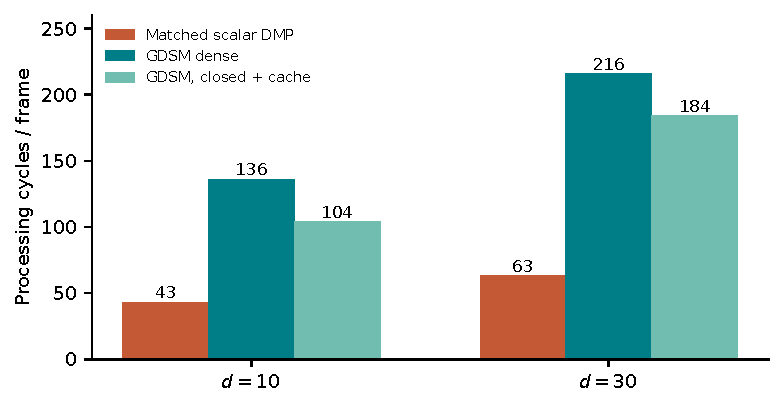
\includegraphics[width=\columnwidth]{figures/hardware.pdf}
\caption{\textbf{Memory-branch processing cycles only.} Cached bars represent fully closed steps. Candidate integration, gating and candidate reading continue, so cached GDSM remains more costly than the matched scalar-DMP branch. These counts do not include the fast spiking backbone and do not measure full-network latency.}
\label{fig:corecycles}
\end{figure}

Figure~\ref{fig:corecycles} retains the measured local costs: 43/63 cycles for scalar DMP at $d=10/30$, 136/216 for dense GDSM, and 104/184 for closed cached GDSM. The full-network operation estimates in Fig.~\ref{fig:hardware} use the Gesture architecture and a different metric; branch-cycle ratios cannot be converted directly into network-level MAC or latency ratios.

\section{Artifact organization and numerical provenance}
\label{app:reproduce}
\paragraph{Evaluation chronology.}
SHD was used iteratively during architecture development, and SSC's official test set had also been evaluated in earlier project stages. For the comparisons reported here, protocols and scheduled checkpoints were fixed before evaluation; the MNIST block froze all 18 models before its official-test evaluation.

The manuscript is built from frozen experiment outputs; preparing this draft introduced no new training runs or checkpoint selection. All primary clean, tail and middle tables and the retention figure are generated directly from archived CSV files. The accompanying artifact contains:
\begin{itemize}[leftmargin=*,itemsep=2pt,topsep=3pt]
\item \texttt{main.tex}, \texttt{references.bib}, generated vector figures and table fragments;
\item \texttt{scripts/build\_assets.py}, which recomputes aggregates and plots without running a model;
\item \texttt{evidence/} copies of metric tables, protocols and the source reports, with SHA-256 provenance in \texttt{source-manifest.json};
\item a machine-readable list of generated numerical claims, citation metadata, and a manuscript audit.
\end{itemize}
Archive paths and checksums are listed in the accompanying evidence map. The Gesture, SSC and MNIST archives retain training protocols, histories, checkpoints and predictions. The hardware archive contains Chisel source, generated RTL, reference traces, waveforms and replay tools.

The hardware trace uses the first official-test S-MNIST image and the seed-42 mixed checkpoint. Its fixed-point gate threshold is $82/4096$ and EMA coefficient $3277/4096$. Cache reuse is checked against dense execution; any open coordinate triggers the full stable read.

\end{document}
